%% LyX 2.3.4.2 created this file.  For more info, see http://www.lyx.org/.
%% Do not edit unless you really know what you are doing.
\documentclass[english,dvipsnames,aspectratio=169,handout]{beamer}
\usepackage{mathptmx}
\usepackage{eulervm}
\usepackage[T1]{fontenc}
\usepackage[latin9]{inputenc}
\usepackage{babel}
\usepackage{amstext}
\usepackage{amssymb}
\usepackage{graphicx}
\usepackage{ifthen}
\usepackage{xcolor}
\usepackage{xspace}
\usepackage{tikz}
\usetikzlibrary{tikzmark}
\usetikzlibrary{calc}
\usepackage{pgfplots}
%\pgfplotsset{compat=1.17}
\usepackage{booktabs}
\usepackage{xpatch}
\usepackage{multirow}
\usepackage{colortbl}
\usepackage{pgfpages}




\xpatchcmd{\itemize}
  {\def\makelabel}
  {\ifnum\@itemdepth=1\relax
     \setlength\itemsep{2ex}% separation for first level
   \else
     \ifnum\@itemdepth=2\relax
       \setlength\itemsep{1ex}% separation for second level
     \else
       \ifnum\@itemdepth=3\relax
         \setlength\itemsep{0.5ex}% separation for third level
   \fi\fi\fi\def\makelabel
  }
 {}
 {}

\ifx\hypersetup\undefined
  \AtBeginDocument{%
    \hypersetup{unicode=true,pdfusetitle,
 bookmarks=true,bookmarksnumbered=false,bookmarksopen=false,
 breaklinks=false,pdfborder={0 0 0},pdfborderstyle={},backref=false,colorlinks=true,
 allcolors=NYUPurple,urlcolor=LightPurple}
  }
\else
  \hypersetup{unicode=true,pdfusetitle,
 bookmarks=true,bookmarksnumbered=false,bookmarksopen=false,
 breaklinks=false,pdfborder={0 0 0},pdfborderstyle={},backref=false,colorlinks=true,
 allcolors=NYUPurple,urlcolor=LightPurple}
\fi

\makeatletter

%%%%%%%%%%%%%%%%%%%%%%%%%%%%%% LyX specific LaTeX commands.
%% Because html converters don't know tabularnewline
\providecommand{\tabularnewline}{\\}

%%%%%%%%%%%%%%%%%%%%%%%%%%%%%% Textclass specific LaTeX commands.
% this default might be overridden by plain title style
\newcommand\makebeamertitle{\frame{\maketitle}}%
% (ERT) argument for the TOC
\AtBeginDocument{%
  \let\origtableofcontents=\tableofcontents
  \def\tableofcontents{\@ifnextchar[{\origtableofcontents}{\gobbletableofcontents}}
  \def\gobbletableofcontents#1{\origtableofcontents}
}

%%%%%%%%%%%%%%%%%%%%%%%%%%%%%% User specified LaTeX commands.
\usetheme{CambridgeUS} 
\beamertemplatenavigationsymbolsempty


% Set Color ==============================
\definecolor{NYUPurple}{RGB}{87,6,140}
\definecolor{LightPurple}{RGB}{165,11,255}


\setbeamercolor{title}{fg=NYUPurple}
\setbeamercolor{frametitle}{fg=NYUPurple}

\setbeamercolor{background canvas}{fg=NYUPurple, bg=white}
\setbeamercolor{background}{fg=black, bg=NYUPurple}

\setbeamercolor{palette primary}{fg=black, bg=gray!30!white}
\setbeamercolor{palette secondary}{fg=black, bg=gray!20!white}
\setbeamercolor{palette tertiary}{fg=gray!20!white, bg=NYUPurple}

\setbeamertemplate{headline}{}
\setbeamerfont{itemize/enumerate body}{}
\setbeamerfont{itemize/enumerate subbody}{size=\normalsize}

\setbeamercolor{parttitle}{fg=NYUPurple}
\setbeamercolor{sectiontitle}{fg=NYUPurple}
\setbeamercolor{sectionname}{fg=NYUPurple}
\setbeamercolor{section page}{fg=NYUPurple}
%\setbeamercolor{description item}{fg=NYUPurple}
%\setbeamercolor{block title}{fg=NYUPurple}

\setbeamertemplate{blocks}[rounded][shadow=false]
\setbeamercolor{block body}{bg=normal text.bg!90!NYUPurple}
\setbeamercolor{block title}{bg=NYUPurple!30, fg=NYUPurple}



\AtBeginSection[]{
  \begin{frame}
  \vfill
  \centering
\setbeamercolor{section title}{fg=NYUPurple}
 \begin{beamercolorbox}[sep=8pt,center,shadow=true,rounded=true]{title}
    \usebeamerfont{title}\usebeamercolor[fg]{title}\insertsectionhead\par%
  \end{beamercolorbox}
  \vfill
  \end{frame}
}

\makeatother

\setlength{\parskip}{\medskipamount} 

\input ../macros

\begin{document}
\input ../rosenberg-macros

%\setbeameroption{show notes on second screen}

\title[DS-GA 1003]{Gaussian Mixture Model}
\author{He He  \\
Slides based on Lecture
\href{https://github.com/davidrosenberg/mlcourse/blob/gh-pages/Lectures/13b.mixture-models.pdf}{13b} from David Rosenberg's course materials (\url{https://github.com/davidrosenberg/mlcourse})
}
\date{April 27, 2021}
\institute{CDS, NYU}

\makebeamertitle
\mode<article>{Just in article version}

\section{Latent Variable Models }
\begin{frame}{General Latent Variable Model}
\begin{itemize}
\item Two sets of random variables: $z$ and $x$.
\item $z$ consists of unobserved \textbf{hidden variables}.
\item $x$ consists of \textbf{observed variables}.

\pause{}
\item Joint probability model parameterized by $\theta\in\Theta$:
\[
p(x,z\mid\theta)
\]
\end{itemize}

\pause{}
\begin{definition}
A\textbf{ latent variable model }is a probability model for which
certain variables are never observed.

\pause{}

\end{definition}

e.g. The Gaussian mixture model is a latent variable model.
\end{frame}

\begin{frame}{Complete and Incomplete Data}
\begin{itemize}
\item Suppose we observe some data $\left(x_{1},\ldots,x_{n}\right)$.

\pause{}
\item To simplify notation, take $x$ to represent the entire dataset
\[
x=\left(x_{1},\ldots,x_{n}\right),
\]
and $z$ to represent the corresponding unobserved variables
\[
z=\left(z_{1},\ldots,z_{n}\right).
\]
\item An observation of $x$ is called an \textbf{incomplete data set}.
\item An observation $\left(x,z\right)$ is called a \textbf{complete data
set}.
\end{itemize}
\end{frame}
%
 
\begin{frame}{Our Objectives}
\begin{itemize}
\item \textbf{Learning problem}: Given incomplete dataset $x$, find MLE
\[
\hat{\theta}=\argmax_{\theta}p(x\mid\theta).
\]


\pause{}
\item \textbf{Inference problem}: Given $x$, find conditional distribution
over $z$:
\[
p\left(z\mid x,\theta\right).
\]


\pause{}
\item For Gaussian mixture model, learning is hard, inference is easy.
\item For more complicated models, inference can also be hard. (See DSGA-1005)
\end{itemize}
\end{frame}
%
\begin{frame}{Log-Likelihood and Terminology}
\begin{itemize}
\item Note that
\[
\argmax_{\theta}p(x\mid\theta)=\argmax_{\theta}\left[\log p(x\mid\theta)\right].
\]


\pause{}
\item Often easier to work with this ``\textbf{log-likelihood}''.

\pause{}
\item We often call $p(x)$ the \textbf{marginal likelihood}, 
\begin{itemize}
\item because it is $p(x,z)$ with $z$ ``marginalized out'':
\[
p(x)=\sum_{z}p(x,z)
\]


\pause{}
\end{itemize}
\item We often call $p(x,z)$ the \textbf{joint}. (for ``joint distribution'')

\pause{}
\item Similarly, $\log p(x)$ is the \textbf{marginal log-likelihood}.
\end{itemize}
\end{frame}
%

\section{EM Algorithm}

\begin{frame}
    {Intuition}
    \head{Problem}: marginal log-likelihood $\log p(x;\theta)$ is hard to optimize (observing only $x$)

    \head{Observation}: complete data log-likelihood $\log p(x,z;\theta)$ is easy to optimize (observing both $x$ and $z$)

    \head{Idea}: guess a distribution of the latent variables $q(z)$ (soft assignments)

    Maximize the \textbf{expected complete data log-likelihood}:
    $$
    \max_\theta \sum_{z\in\sZ} q(z) \log p(x,z;\theta)
    $$

    \head{EM assumption}: the expected complete data log-likelihood is easy to optimize

    Why should this work?
\end{frame}

\section{Math Prerequisites}

\begin{frame}{Jensen's Inequality}

\begin{theorem}
[Jensen's Inequality]If $f:\reals\to\reals$ is a \textbf{convex}
function, and $x$ is a random variable, then
\[
\ex f(x)\ge f(\ex x).\pause
\]
Moreover, if $f$ is \textbf{strictly convex}, then equality implies
that $x=\ex x$ with probability $1$ (i.e. $x$ is a constant).
\end{theorem}


\pause{}
\begin{itemize}
\item e.g. $f(x)=x^{2}$ is convex. So $\ex x^{2}\ge\left(\ex x\right)^{2}$.
Thus 
\[
\var\left(x\right)=\ex x^{2}-\left(\ex x\right)^{2}\ge0.
\]
 
\end{itemize}
\end{frame}
%
\begin{frame}{Kullback-Leibler Divergence}

\begin{itemize}
\item Let $p(x)$ and $q(x)$ be probability mass functions (PMFs) on $\cx$. 
\item How can we measure how ``different'' $p$ and $q$ are?
\end{itemize}

\pause{}
\begin{itemize}
\item The \textbf{Kullback-Leibler} or \textbf{``KL'' Divergence} is defined
by
\begin{eqnarray*}
\kl(p\|q) & = & \sum_{x\in\cx}p(x)\log\frac{p(x)}{q(x)}.
\end{eqnarray*}
(Assumes $q(x)=0$ implies $p(x)=0$.)
\end{itemize}

\pause{}
\begin{itemize}
\item Can also write this as
\begin{eqnarray*}
\kl(p\|q) & = & \ex_{x\sim p}\log\frac{p(x)}{q(x)}.
\end{eqnarray*}
\end{itemize}
\end{frame}
%
\begin{frame}{Gibbs Inequality ($\kl(p\|q)\ge0$ and $\kl(p\|p)=0$)}
\begin{theorem}
[Gibbs Inequality]Let $p(x)$ and $q(x)$ be PMFs on $\cx$. Then
\[
\kl(p\|q)\ge0,
\]
with equality iff $p(x)=q(x)$ for all $x\in\cx$. 
\end{theorem}


\pause{}
\begin{itemize}
\item KL divergence measures the ``distance'' between distributions.
\end{itemize}

\pause{}
\begin{itemize}
\item Note:

\begin{itemize}
\item KL divergence \textbf{not a metric}.
\item KL divergence is \textbf{not symmetric}.
\end{itemize}
\end{itemize}
\end{frame}
%
\begin{frame}{Gibbs Inequality: Proof}

\begin{eqnarray*}
\kl(p\|q) & = & \ex_{p}\left[-\log\left(\frac{q(x)}{p(x)}\right)\right]\\
 & \ge & -\log\left[\ex_{p}\left(\frac{q(x)}{p(x)}\right)\right]\mbox{\qquad\text{(Jensen's)}}\\
 & = & -\log\left[\sum_{\left\{ x\mid p(x)>0\right\} }p(x)\frac{q(x)}{p(x)}\right]\\
 & = & -\log\left[\sum_{x\in\cx}q(x)\right]\\
 & = & -\log1=0.
\end{eqnarray*}


\pause{}
\begin{itemize}
\item Since $-\log$ is strictly convex, we have strict equality iff $q(x)/p(x)$
is a constant, which implies $q=p$ . 
\end{itemize}
\end{frame}

\section{The ELBO: Family of Lower Bounds on $\log p(x\mid\theta)$}
\begin{frame}{The Maximum Likelihood Estimator}

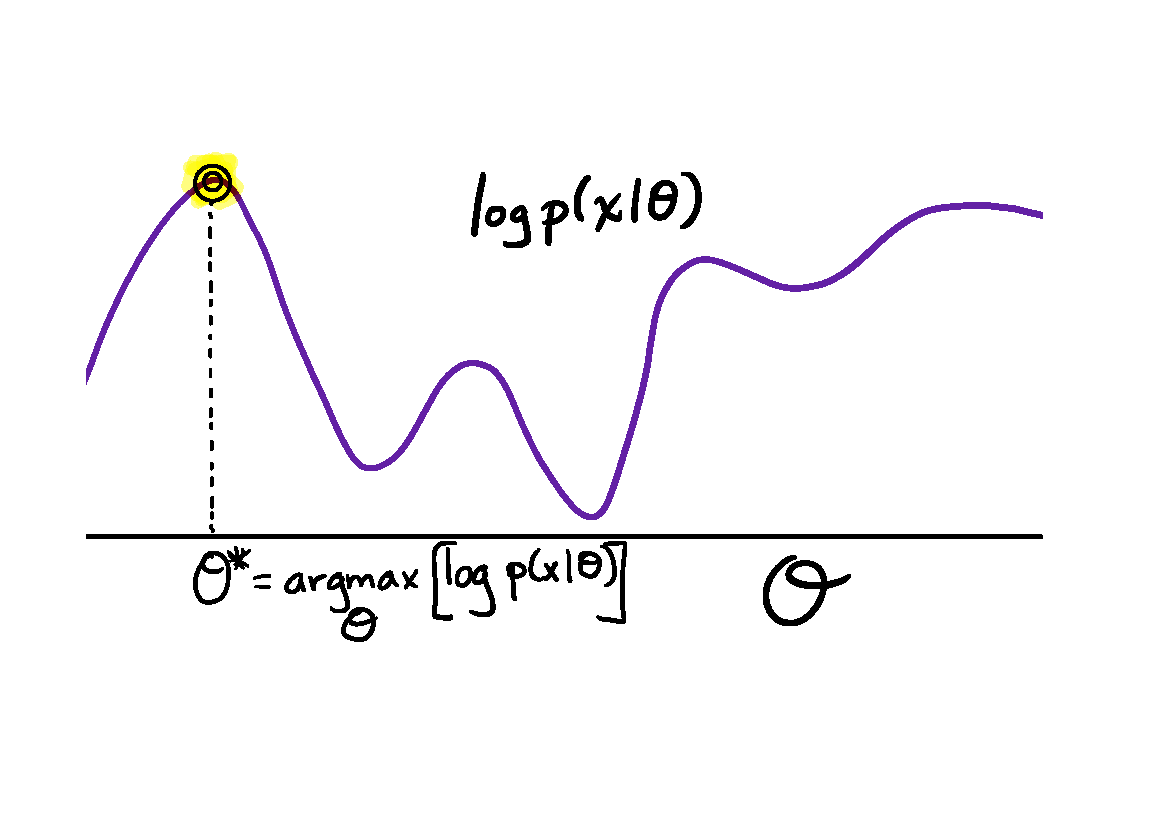
\includegraphics[width=0.85\textwidth]{figures/margLL-withMax.pdf}
\end{frame}

\begin{frame}
    {Lower bound of the marginal log-likelihood}
    \begin{align*}
        \log p(x;\theta) &= \log \sum_{z\in\sZ} p(x,z;\theta) \\
        &= \log \sum_{z\in\sZ} q(z) \frac{p(x,z;\theta)}{q(z)}\\
        %\quad {\color{brown}= \log \BE_z\pb{p(x,z;\theta)}}\\
        &\ge \sum_{z\in\sZ} q(z) \log \frac{p(x,z;\theta)}{q(z)}\\
        %\quad {\color{brown}= \BE_z\pb{\log p(x,z;\theta)}} \\
        &\eqdef \sL(q, \theta)
    \end{align*}
    \vspace{-2em}
    \begin{itemize}
        \setlength\itemsep{2pt}
        \item \textbf{Evidence}:  $\log p(x;\theta)$
        \item \textbf{Evidence lower bound (ELBO)}: $\sL(q, \theta)$
        \item $q$: chosen to be a family of tractable distributions
        \item Idea: \emph{maximize the ELBO} instead of $\log p(x;\theta)$
    \end{itemize}
\end{frame}

\begin{frame}{MLE, EM, and the ELBO}
\begin{itemize}
\item The MLE is defined as a maximum over $\theta$:
\[
\hat{\theta}_{\text{MLE}}=\argmax_{\theta}\left[\log p(x\mid\theta)\right].
\]
\item For any PMF $q(z)$, we have a lower bound on the marginal log-likelihood
\[
\log p(x\mid\theta)\ge\cl(q,\theta).
\]
\item In EM algorithm, we maximize the lower bound (ELBO) over $\theta$
and $q$:
\[
\hat{\theta}_{\text{EM}}\approx\argmax_{\theta}\left[\max_{q}\cl(q,\theta)\right]
\]
\end{itemize}

\pause{}
\begin{itemize}
\item In EM algorithm, $q$ ranges over all distributions on $z$.
\end{itemize}
\end{frame}

\begin{frame}{EM: Coordinate Ascent on Lower Bound}
\begin{itemize}
\item Choose sequence of $q$'s and $\theta$'s by ``\textbf{coordinate
ascent}'' on $\cl(q,\theta)$.

\pause{}
\item EM Algorithm (high level):
\begin{enumerate}
\item Choose initial $\theta^{\text{old}}$.
\item Let $q^{*}=\argmax_{q}\cl(q,\theta^{\text{old}})$

\pause{}
\item Let $\theta^{\text{new}}=\argmax_{\theta}\cl(q^{*},\theta^{\text{old}})$.

\pause{}
\item Go to step 2, until converged.
\end{enumerate}
\item Will show:\textbf{ $p(x\mid\theta^{\text{new}})\ge p(x\mid\theta^{\text{old}})$}
\item \textbf{Get sequence of $\theta$'s with monotonically increasing
likelihood.}
\end{itemize}
\end{frame}

\begin{frame}{EM: Coordinate Ascent on Lower Bound}
\begin{center}
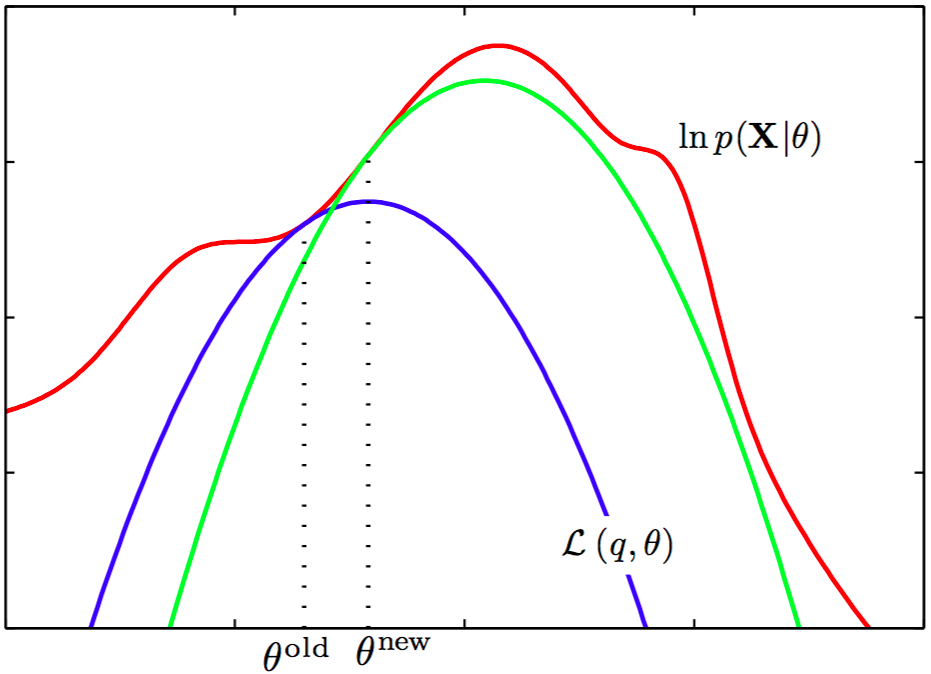
\includegraphics[height=0.5\textheight]{figures/EM-twosteps-Bishop9.14.png} 
\par\end{center}
\begin{enumerate}
\item Start at $\theta^{\text{old}}.$ 

\pause{}
\item Find $q$ giving best lower bound at $\theta^{\text{old}}$$\implies$
$\cl(q,\theta)$. 

\pause{}
\item $\theta^{\text{new}}=\argmax_{\theta}\cl(q,\theta)$.
\end{enumerate}
\let\thefootnote\relax\footnotetext{\tiny{From Bishop's \emph{Pattern recognition and machine learning}, Figure 9.14.}}
\end{frame}

\begin{frame}
    {Justification for maximizing ELBO}
    \begin{align*}
        \sL(q, \theta) &= \sum_{z\in\sZ} q(z) \log \frac{p(x,z;\theta)}{q(z)} \\
        &= \sum_{z\in\sZ} q(z)\log \frac{p(z\mid x;\theta)p(x;\theta)}{q(z)} \\
        &= -\sum_{z\in\sZ}q(z) \log \frac{q(z)}{p(z\mid x;\theta)}
        + \sum_{z\in\sZ} q(z) \log p(x;\theta) \\
        &= -\KL{q(z)}{p(z\mid x;\theta)} + \underbrace{\log p(x;\theta)}_{\text{evidence}}
    \end{align*}
    \vspace{-2em}
    \begin{itemize}
        \item \textbf{KL divergence}: measures ``distance'' between two distributions (not symmetric!)
        \item $\KL{q}{p}\ge 0$ with equality iff $q(z) = p(z\mid x)$.
        \item ELBO = evidence - KL $\le$ evidence
    \end{itemize}
\end{frame}

\begin{frame}{Maximizing over $q$ for fixed $\theta$.}
\begin{itemize}
\item Find $q$ maximizing
\begin{eqnarray*}
\cl(q,\theta) & = & -\kl[q(z),p(z\mid x,\theta)]+\underbrace{\log p(x\mid\theta)\pause}_{\text{no }q\text{ here}}
\end{eqnarray*}


\pause{}
\item Recall $\kl(p\|q)\ge0$, and $\kl(p\|p)=0$.

\pause{}
\item Best $q$ is $q^{*}(z)=p(z\mid x,\theta)$ and
\[
\pause\cl(q^{*},\theta)=-\underbrace{\kl[p(z\mid x,\theta),p(z\mid x,\theta)]}_{=0}+\log p(x\mid\theta)
\]


\pause{}
\item Summary:
\[
\log p(x\mid\theta)=\sup_{q}\cl(q,\theta)\qquad\forall\theta
\]
\item For any $\theta$, \textbf{sup is attained} at $q(z)=p(z\mid x,\theta)$. 
\end{itemize}
\end{frame}
%

%\begin{frame}
%    {\dis Justification for maximizing ELBO}
%    $
%    \sL(q, \theta) = -\KL{q(z)}{p(z\mid x;\theta)} + \log p(x;\theta)
%    $
%
%    Fix $\theta=\theta_0$ and $\max_q \sL(q, \theta_0)$: $q^* = p(z\mid x;\theta_0)$ 
%    \vspace{10em}
%
%    Let $\theta^*, q^*$ be the global optimzer of $\sL(q, \theta)$, then $\theta^*$ is the global optimizer of $\log p(x;\theta)$. (Proof: exercise)
%\end{frame}

\begin{frame}{Marginal Log-Likelihood \textbf{IS}\textbf{\textcolor{blue}{\LARGE{}
}}the Supremum over Lower Bounds}

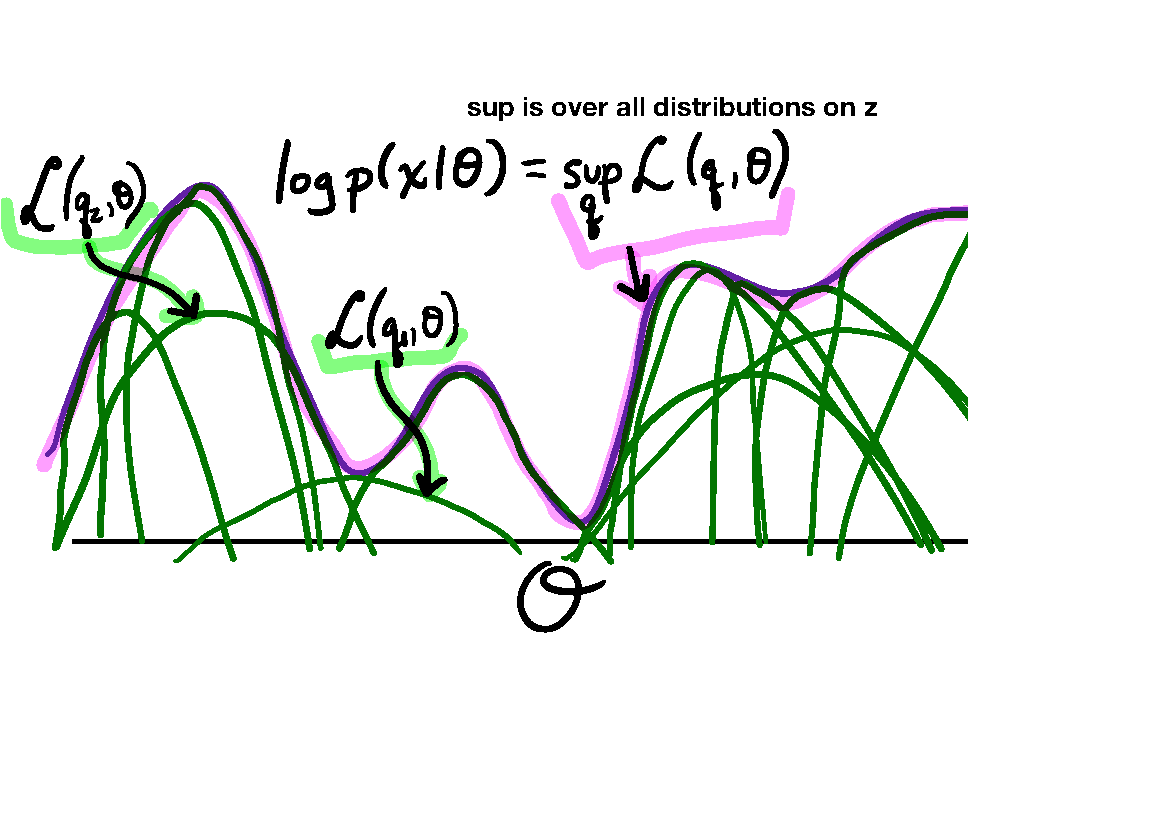
\includegraphics[width=0.75\textwidth]{figures/sup-margLL.pdf} 
\end{frame}

\begin{frame}
    {Summary}
    \textbf{Latent variable models}: clustering, latent structure, missing lables etc.

    \head{Parameter estimation}: maximum marginal log-likelihood

    \head{Challenge}: directly maximize the \textbf{evidence} $\log p(x;\theta)$ is hard

    \head{Solution}: maximize the \textbf{evidence lower bound}:
    $$
    \text{ELBO} = \sL(q, \theta) = -\KL{q(z)}{p(z\mid x;\theta)} + \log p(x;\theta)
    $$

    \head{Why does it work?}
    \begin{align*}
        q^*(z) &= p(z\mid x; \theta) \quad \forall \theta \in \Theta \\
        \sL(q^*, \theta^*) &= \max_\theta \log p(x; \theta)
    \end{align*}
\end{frame}

\begin{frame}
    {EM algorithm}
    \emph{Coordinate ascent on $\sL(q, \theta)$}\\
    \begin{enumerate}
        \item Random initialization: $\theta^{\text{old}} \leftarrow \theta_0$
        \item Repeat until convergence
            \begin{enumerate}[(i)]
                \item $q(z) \leftarrow \argmax_q \sL(q, \theta^{\text{old}})$
                    \begin{align*}
                    \text{\textbf{Expectation} (the E-step):} \quad
                    q^*(z) &= p(z\mid x;\theta^{\text{old}}) \\
                        J(\theta) &= \sL(q^*, \theta) 
                    \end{align*}
                \item $\theta^{\text{new}} \leftarrow \argmax_\theta \sL(q^*, \theta)$
                    \begin{align*}
                        \text{\textbf{Maximization} (the M-step):} \quad
                        \theta^{\text{new}} \leftarrow \argmax_\theta J(\theta)
                    \end{align*}
            \end{enumerate}
    \end{enumerate}
\end{frame}

\begin{frame}{EM Algorithm}
\begin{enumerate}
%\item Choose initial $\theta^{\text{old}}$.
\item \textbf{Expectation Step}
\begin{itemize}
    \setlength\itemsep{1pt}
\item Let $q^{*}(z)=p(z\mid x,\theta^{\text{old}})$. {[}$q^{*}$ gives
best lower bound at $\theta^{\text{old}}${]}

\pause{}
\item Let
\[
J(\theta):=\cl(q^{*},\theta)=\underbrace{\sum_{z}q^{*}(z)\log\left(\frac{p(x,z\mid\theta)}{q^{*}(z)}\right)}_{\mbox{\textbf{expectation }w.r.t. }z\sim q^{*}(z)}
\]
 

\pause{}
\end{itemize}
\item \textbf{Maximization Step} 
\[
\theta^{\text{new}}=\argmax_{\theta}J(\theta).\pause
\]
{[}Equivalent to maximizing expected complete log-likelihood.{]}

\pause{}
%\item Go to step 2, until converged.
\end{enumerate}
        EM puts no constraint on $q$ in the E-step and assumes the M-step is easy.
        In general, both steps can be hard.
\end{frame}

\begin{frame}
    {\dis Monotonically increasing likelihood}
    \begin{figure}
        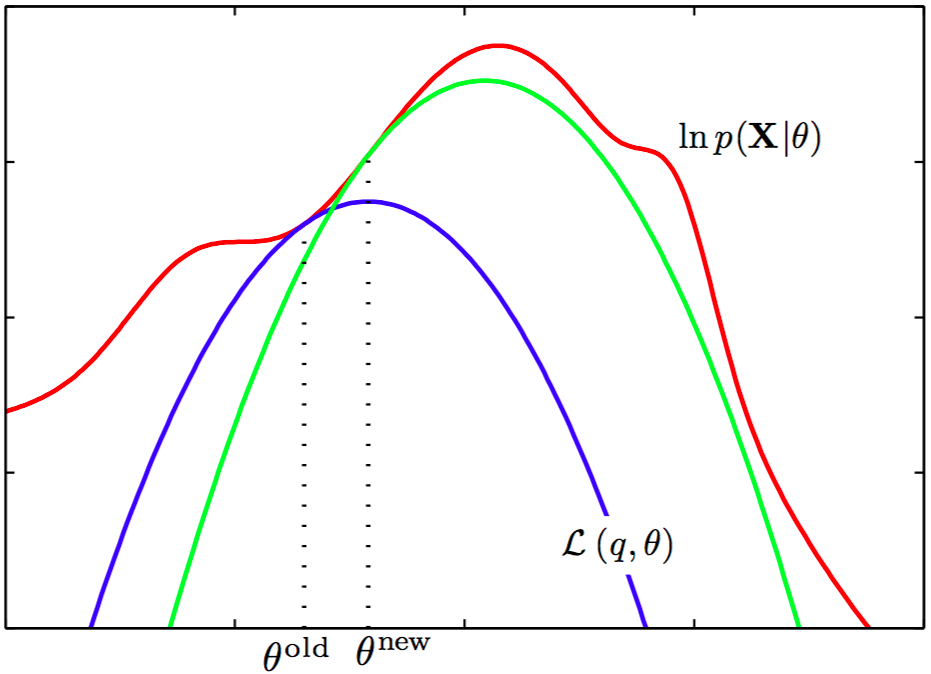
\includegraphics[height=5cm]{figures/EM-twosteps-Bishop9.14.png}
    \end{figure}
    \vspace{-2em}
    Exercise: prove that EM increases the marginal likelihood monotonically
    $$
    \log p(x;\theta^{\text{new}}) \ge \log p(x;\theta^{\text{old}})
    \;.
    $$
    Does EM converge to a global maximum?
\end{frame}

\section{Variations on EM}

\begin{frame}{EM Gives Us Two New Problems}
\begin{itemize}
\item The ``E'' Step: Computing

\[
J(\theta):=\cl(q^{*},\theta)=\sum_{z}q^{*}(z)\log\left(\frac{p(x,z\mid\theta)}{q^{*}(z)}\right)
\]


\pause{}
\item The ``M'' Step: Computing
\[
\theta^{\text{new}}=\argmax_{\theta}J(\theta).\pause
\]


\pause{}
\item Either of these can be too hard to do in practice.
\end{itemize}
\end{frame}

\begin{frame}{Generalized EM (GEM)}
\begin{itemize}
\item Addresses the problem of a difficult ``M'' step.

\pause{}
\item Rather than finding 
\[
\theta^{\text{new}}=\argmax_{\theta}J(\theta),
\]
find \textbf{any} $\theta^{\mbox{new}}$ for which
\[
J(\theta^{\mbox{new}})>J(\theta^{\mbox{old}}).
\]


\pause{}
\item Can use a standard nonlinear optimization strategy
\begin{itemize}
\item e.g. take a gradient step on $J$.

\pause{}
\end{itemize}
\item We still get monotonically increasing likelihood. 
\end{itemize}
\end{frame}

\begin{frame}{EM and More General Variational Methods}
\begin{itemize}
\item Suppose ``E'' step is difficult:
\begin{itemize}
\item Hard to take expectation w.r.t. $q^{*}(z)=p(z\mid x,\theta^{\text{old}})$.
\end{itemize}

\pause{}
\item Solution: Restrict to distributions $\cq$ that are easy to work with. 

\pause{}
\item Lower bound now looser:
\[
q^{*}=\argmin_{q\in\cq}\kl[q(z),p(z\mid x,\theta^{\text{old}})]
\]
\end{itemize}
\end{frame}

\end{document}
